% Working draft based on the approved Chinese manuscript and author revisions.
% 2026-11-08: Method (3), Listening Data Construction (4), Experiments (5).
% Task is nested in Method; evaluation remains nested in Experiments.
% Compile with XeLaTeX. Chinese author notes are intentionally visible.
\documentclass[10pt,twocolumn,letterpaper]{article}
\usepackage[review]{cvpr}
\usepackage{xeCJK}
% Load TeX Live Fandol by filename. Name-only lookup fails on some Mac setups
% without fontconfig, even when the OTF files are present in texmf-dist.
\setCJKmainfont[
  Extension=.otf,
  BoldFont=FandolSong-Bold,
]{FandolSong-Regular}
\setCJKsansfont[
  Extension=.otf,
  BoldFont=FandolHei-Bold,
]{FandolHei-Regular}
\usepackage{tabularx,array,makecell}
\usepackage{placeins}
\definecolor{cvprblue}{rgb}{0.21,0.49,0.74}
\definecolor{authorblue}{RGB}{40,81,125}
\newif\ifauthornotes
\authornotestrue
% Chinese planning notes: keep visible in this authoring draft.
\newcommand{\cnnote}[2]{\ifauthornotes\par\smallskip{\small\upshape\color{authorblue}\noindent\textbf{【#1】}#2\par}\smallskip\fi}
\newcommand{\pending}{\textcolor{authorblue}{\textsf{TBD}}}
\newcommand{\NA}{\textsf{N/A}}
\newcommand{\on}{\ensuremath{\checkmark}}
\newcommand{\off}{\ensuremath{-}}
\newcolumntype{Y}{>{\raggedright\arraybackslash}X}
\newcommand{\figdraft}[1]{\textbf{#1 (draft).}}
\graphicspath{{figures/}}
% Do not hide layout defects behind the template's 30pt tolerance.
\hfuzz=0pt
\vfuzz=0pt

\usepackage[pagebackref,breaklinks,colorlinks,allcolors=cvprblue]{hyperref}
\def\confName{CVPR}
\def\confYear{2027}
\title{Audiovisual Backchannel Generation During Listening}
\author{Anonymous Authors}
\begin{document}
\maketitle
\begin{abstract}
\cnnote{摘要待写}{按中文稿约定，待主张、正式实验和结果稳定后撰写摘要。当前标题只用于识别任务，尚非最终标题。本版为英文正文与中文作者备注并存的工作稿；表中的TBD表示尚未填写，不代表零分；图中示意素材不作为实验结果。}
\end{abstract}

% 2026-11-08: revised from the author's version, not from the initial draft.
% Exact author version and change rationale: review/intro_revision_20261108/.
% Citation keys are stable placeholders; replace matching entries in references.bib.
\section{Introduction}
\label{sec:intro}

% Paragraph role P01: 任务价值与成功标准——倾听行为是否合适，而不仅是媒体是否逼真。
Natural conversation requires both speaking and listening. While one
participant holds the conversational floor, the listener conveys attention
and engagement through facial expressions, head movements, and brief vocal
acknowledgments~\cite{learningtolisten,omnipersona}. These backchannels
support the ongoing utterance without taking over the conversation. Visual
reactions may occur with or without vocal feedback, and quiet listening is
also appropriate. Digital humans therefore need to produce appropriate
listening behavior as well as fluent spoken responses: realistic faces and
voices alone do not establish whether feedback fits the conversational
context.

\begin{figure*}[t]
\centering
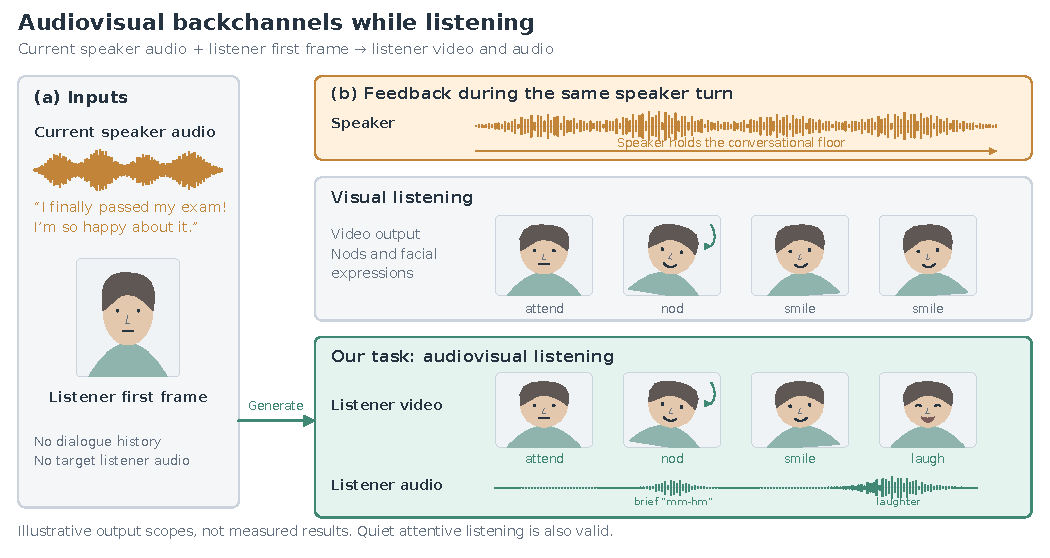
\includegraphics[width=\textwidth]{F1_task.pdf}
\caption{\figdraft{F1: Audiovisual backchannels during listening} Given current speaker audio and the listener's first frame, the task is to generate listener video and audio while the speaker holds the floor. Quiet listening is also valid. The rows illustrate visual and audiovisual output scopes, not measured comparisons between methods. Portraits, utterances, and waveforms are schematic.}
\label{fig:task}
\end{figure*}

% Paragraph role P02: 已有能力递进——给定目标语音、视觉倾听、双音轨交互、自主视听回应。
Speech-driven talking-head methods such as
OmniHuman-1.5~\cite{omnihuman15} synthesize visual behavior from the target
person's supplied speech. Listening-generation methods, including
ViCo~\cite{vico}, Learning to Listen~\cite{learningtolisten}, and
GLARE~\cite{glare}, instead generate visual reactions to another speaker
without synthesizing the listener's audio. 
% GLARE also introduces reaction-oriented supervision and evaluation.
Interactive methods such as INFP~\cite{infp} and DyStream~\cite{dystream}
model speaking and listening from both participants' audio tracks, with
the target person's vocal behavior supplied as an input. OmniResponse~\cite{omniresponse}
and OmniPersona~\cite{omnipersona} further generate audiovisual
conversational responses, including listener feedback. Building on these
advances, we focus on listening feedback as the primary target of learning
and evaluation, and investigate how listening-specific conditioning,
supervision, and data can support its visual and vocal expression.
% 引用边界：不推断OmniResponse／OmniPersona只做整段对话评价；两者已有倾听反馈研究。

% Paragraph role P03: 任务设定及应用理由——无需用户视频，允许无历史的初次／独立交流。
We study audiovisual backchannel generation from the current speaker audio
and a reference image of the listener (\cref{fig:task}). This setting
supports interaction with a visible digital avatar without requiring the
user to enable a camera, and accommodates initial or standalone exchanges
with no prior dialogue history. 
% The image specifies the avatar's visual identity, while the current utterance provides the conversational input.
The listener's audio is generated rather than supplied: the model must
produce visual reactions, brief vocal feedback, and quiet listening while
the speaker retains the floor.

% Paragraph role P04: 两个建模挑战——从对方语音构建生成条件，以及显式监督短暂反馈行为。
Learning this behavior presents two related challenges. First, the input
speech belongs to the other participant: it provides semantic and acoustic
cues, but does not prescribe the listener's articulation or reaction.
These cues must be mapped to conditions suitable for generating the
listener's audio and video. Second, feedback can be brief, subtle, and
interspersed with quiet listening. A media-generation objective supervises
the audiovisual output as a whole, but does not explicitly specify which
feedback categories should occur. This motivates event supervision that
makes feedback behavior a direct target of learning.
% 这是本文的设计依据，不是对所有既有模型已验证的失败结论。

% Paragraph role P05: 方法回应挑战——直接声学条件＋目标特征适配，对应第一个挑战；Event对应第二个。
Our framework addresses these challenges through direct speaker-audio
conditioning and supervision of both conditioning representations and
feedback events. Speaker-audio cross-attention supplies acoustic
information to the generator, while target audiovisual feature supervision
trains the conditioning mapping to retain information relevant to the
listener's response. Clip-level event supervision complements the
media-generation objective by encouraging the corresponding feedback
categories to occur. This auxiliary objective supervises category presence
over the clip without imposing exact event timestamps.
% Feature监督适配条件映射，不更新冻结Qwen；整段Event不表示其他AV训练目标也放弃时间对应。
% 效果待证据：上述句子说明机制与目标，不预填组件收益或联合优于级联的结论。

% Paragraph role P06: 数据回应学习要求——角色更新、配对媒体和有序视听反应描述。
To support listening-focused learning, we construct paired
audiovisual data from Seamless conversations~\cite{seamless},
updating speaker--listener roles as turns change while retaining
brief vocal backchannels as listening feedback. We use extracted
visual and vocal cues to guide Qwen3-Omni~\cite{qwen3omni} in
producing ordered reaction descriptions, linking speaker audio
with listener audiovisual media and annotations of their feedback.

% Paragraph role P07: 评价回应任务标准——类别一致性、语境／参与感、生成音画自身协调。
We formulate a listening-focused evaluation design that considers
audiovisual quality, feedback-category agreement, contextual
appropriateness and engagement, and audiovisual coordination. A speaker
utterance can admit multiple reasonable reactions~\cite{learningtolisten,reactface},
so agreement with one recorded response cannot fully determine feedback
quality. Clip-level category agreement measures whether the reference
feedback categories are expressed without requiring temporal overlap with
reference events. Contextual evaluation considers whether a response fits
the utterance and preserves the listening role, including reasonable
alternatives to the reference; audiovisual coordination concerns the
relation between generated sounds and movements. Together, these
dimensions separate media quality from the listening behavior it conveys.
% GLARE也承认一对多；这里的区别是类别一致性不要求时间重叠，不是首次提出一对多。
% 后续计划仍为中文：类别／检测器、人工量表及正式结果未定，故使用evaluation design。

% Paragraph role P08: 贡献收束——保留作者的模型、数据、评价顺序。
Our contributions are as follows:
\begin{itemize}
    \item We introduce an audiovisual backchannel generation framework
    conditioned on current speaker audio and a listener reference image.
    It combines direct acoustic conditioning, target audiovisual feature
    supervision, and clip-level event supervision for listening feedback.

    \item \textcolor{red}{(如果写数据贡献，需要一些体现贡献的数字：xxh，xxpairs，xxtypes…)}We construct listening-focused audiovisual data through
    role-aware clip pairing and cue-assisted feedback annotation,
    associating speaker audio with listener audiovisual media and ordered
    descriptions of visual and vocal behavior.

    \item We formulate a listening-focused evaluation design that
    complements audiovisual quality with feedback-category agreement,
    contextual appropriateness and engagement, and audiovisual
    coordination, accommodating reasonable variation in listener responses.
\end{itemize}




% 11-07
% \section{Introduction}
% \label{sec:intro}
% % Paragraph role P01: 开场：任务及目标
% Speakers and listeners both contribute to natural conversation. Listeners use nods, facial expressions, and brief vocal acknowledgments to convey attention and engagement. Digital humans therefore need to produce natural audiovisual feedback while listening. We study audiovisual backchannel generation from the current speaker audio and a reference image of the listener, with the aim of making conversation more natural and engaging (\cref{fig:task}).

% \begin{figure*}[t]
% \centering
% 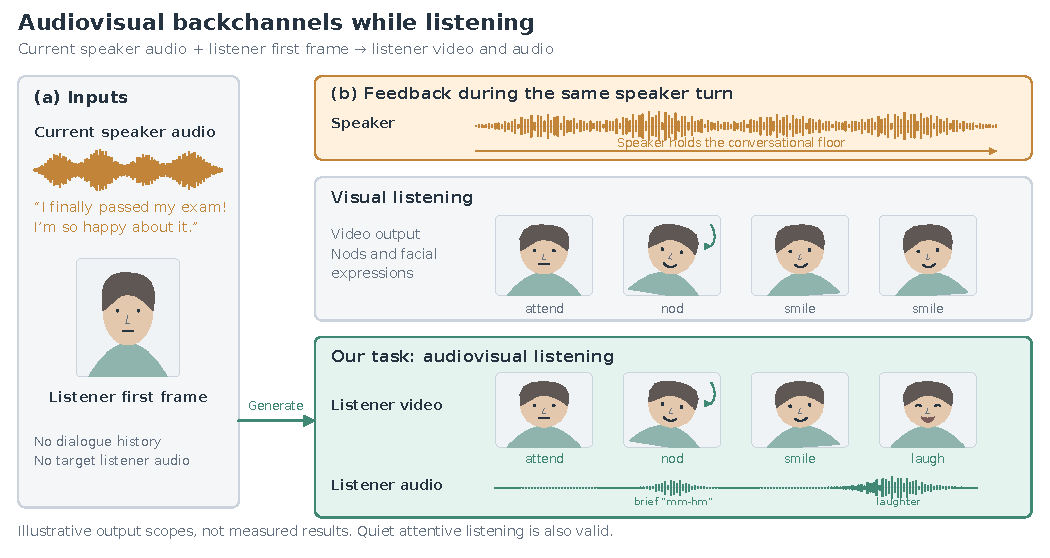
\includegraphics[width=\textwidth]{F1_task.pdf}
% \caption{\figdraft{F1: Audiovisual backchannels during listening} Given current speaker audio and the listener's first frame, the task is to generate listener video and audio while the speaker holds the floor. Quiet listening is also valid. The rows illustrate visual and audiovisual output scopes, not measured comparisons between methods. Portraits, utterances, and waveforms are schematic.}
% \label{fig:task}
% \end{figure*}

% % Paragraph role P02: 已有能力与本文范围
% Speech-driven talking-head methods, such as OmniHuman-1.5~\cite{omnihuman15}, generate facial motion from the target person's given speech, emphasizing lip synchronization and natural motion. Listening-generation methods instead model responses to a speaker. ViCo~\cite{vico}, Learning to Listen~\cite{learningtolisten}, and GLARE~\cite{glare} generate visual listening behavior without generating the listener's own audio. More recent work, including OmniResponse~\cite{omniresponse} and OmniPersona~\cite{omnipersona}, also studies vocal and silent responses. We focus on feedback produced while the speaker holds the conversational floor, using only the current speaker audio and the listener's reference image, without dialogue history or a supplied listener audio track.

% % Paragraph role P03: 技术困难与设计目标
% This task requires converting semantic and acoustic information in the current speech into listener sounds and visual behavior. General multimodal representations provide a basis for understanding, but their mapping to audiovisual generation conditions still needs to be adapted to listening. Moreover, media reconstruction objectives do not directly specify whether feedback categories, such as nods or acknowledgments, should occur. We therefore address the use of current speech information, the adaptation of conditioning representations, and explicit supervision of feedback behavior.

% % Paragraph role P04: 数据需求
% The task also requires paired speaker inputs, listener video, and the listener's own audio, with clear listening roles and feedback annotations. Existing resources support these requirements to different extents. Some do not provide an independent listener audio track ready for generation training. Others contain both participants' audiovisual information but still require listening-oriented sample organization and backchannel annotation. Converting raw conversations into suitable training samples thus requires task-specific data preparation.
% \cnnote{待补引用}{上述资源差异沿用中文稿的限定表述。定稿时须为各类局限补充对应资源证据；不将Seamless或ResponseNet写成完全没有音轨或行为标注。}

% % Paragraph role P05: 评价需求
% Evaluation must also address listening behavior. Standard video-quality metrics describe visual fidelity and realism, but a visually convincing output may still lack meaningful feedback or respond inappropriately to the current utterance. Evaluation should therefore consider audiovisual quality, feedback behavior, naturalness, and conversational engagement.

% % Paragraph role P06: 数据方案
% We address these requirements through data construction, a generation framework, and an evaluation design. Starting from Seamless conversations~\cite{seamless}, we use pauses, ASR punctuation, and transcript-based utterance-boundary cues to organize paired speaker--listener clips. To address reaction omissions observed when describing audiovisual clips directly, we extract visual and vocal cues and provide their categories and temporal intervals to Qwen3-Omni~\cite{qwen3omni}. The resulting natural-language descriptions organize reactions in their observed order, providing paired media and descriptions for learning audiovisual listening responses.

% % Paragraph role P07: 方法方案
% Our generator uses speaker-audio cross-attention to supply direct acoustic information, target audiovisual feature supervision to adapt the conditioning representations, and clip-level event supervision to encourage the corresponding backchannel categories. These components address input information, condition adaptation, and feedback expression, respectively.
% \cnnote{证据待补}{这里陈述设计目的；三个组件的实际效果由最终同条件消融支持，不预写显著提升或最优结论。}

% % Paragraph role P08: 评价方案
% Our evaluation design considers clip-level event-category agreement, contextual appropriateness and engagement, and audiovisual event coordination. Category agreement allows feedback timing to vary, contextual evaluation allows different reasonable responses, and coordination concerns the relation between generated sounds and movements.
% \cnnote{协议待补}{测试集组织、事件检测与核验、人工评价工具及细则尚待确定；不表示完整benchmark已执行或发布。}

% % Paragraph role P09: 贡献入口
% Our contributions are as follows:
% \begin{itemize}
% \item We construct paired data for audiovisual backchannel generation during listening from Seamless conversations. Role-aware clip organization, media processing, and cue-assisted annotation link speaker audio, listener audiovisual media, and ordered reaction descriptions.
% \item We introduce a generation framework conditioned on current speaker audio and the listener's first frame. Direct audio conditioning supplies acoustic information, target feature supervision adapts the conditioning representations, and clip-level event supervision explicitly encourages feedback categories.
% \item We organize feedback evaluation around clip-level category agreement, contextual appropriateness and engagement, and audiovisual coordination, complementing media-quality evaluation while allowing reasonable variation in reaction timing.
% \end{itemize}
% \cnnote{贡献边界}{第三条保留为已确认的评价设计，不新增“首个”“首次”或“已发布benchmark”的主张。本文仅说明采用联合生成，不主张其已被证明优于音频—视频级联。}

\section{Related Work}
\label{sec:related}
\subsection{Audiovisual Conversation and Response Generation}
% Paragraph role P01: 视觉倾听沿革
Listening-generation methods synthesize facial expressions and head movements from a speaker's communication signals. ViCo~\cite{vico} introduces responsive listening-head generation and paired data, using speaker audiovisual signals and a preset attitude to generate listener motion. Learning to Listen~\cite{learningtolisten} models listener motion as a nondeterministic distribution, allowing multiple responses to the same input. Subsequent work explores diffusion-based diverse generation, emotion control, and text-based customization through MFR-Net~\cite{mfrnet}, ELP~\cite{elp}, and CustomListener~\cite{customlistener}, respectively. DiffListener~\cite{difflistener} and DiTaiListener~\cite{ditailistener} further develop expressive listening-video generation.

% Paragraph role P02: 行为适当性与事件表示
Beyond visual quality, ReactFace~\cite{reactface} studies online generation of multiple appropriate facial reactions, considering appropriateness, diversity, and synchrony. GLARE~\cite{glare} represents reactions as events with categories and temporal intervals, combining prosodic conditioning, temporal reaction supervision, and event evaluation. These visual listening methods provide a basis for behavior modeling, but do not generate the listener's own audio. Our task includes brief acknowledgments and laughter together with the corresponding video, while retaining silent listening as a valid output.

% Paragraph role P03: 已知音轨的交互视频
Interactive-avatar methods also differ in whether the target audio is supplied or generated. INFP~\cite{infp} and DyStream~\cite{dystream} use both participants' audio tracks to generate avatar videos that include speaking and listening. ARIG~\cite{arig} additionally models interaction using both participants' audiovisual signals and dialogue states. These methods incorporate role changes and listening into generation, but receive the target person's audio as a condition. Our model must generate both listener audio and video from the other person's current speech and a listener reference frame.

% Paragraph role P04: 自主AV回应与本文边界
OmniResponse~\cite{omniresponse} is closer to this setting: it uses speaker facial information, transcripts, and dialogue history to generate aligned text and facial responses, with TempoVoice synthesizing audio for vocal responses. OmniPersona~\cite{omnipersona} encodes multimodal conversation history into linguistic and non-linguistic conditions and jointly generates audio and video, including listening backchannels and identity consistency across turns. Audiovisual listening responses therefore already have a research basis. Our focus is feedback during the other person's turn from a short current audio segment and a listener first frame, without dialogue history, speaker video, a target listener audio track, or a reference voice. We address this setting through direct audio conditioning, target feature supervision, and clip-level event supervision, rather than introducing a multi-turn memory task.

\subsection{MLLM-Based Cascaded Generation}
% \cnnote{中文待补：作者已确认的新结构}{本小节尚无写定正文，先保留中文。后续结合OmniPersona对理解与生成框架的介绍，核实“MLLM理解／规划→文本或隐表征→生成器”的代表工作、接口与条件，再写文献介绍。不能把所有条件接口统称为同一种级联；Qwen→OVI系统对照也不等于先生成音频再驱动视频。这里不新增“联合生成优于级联”的主张，暂不补造文献或技术关系。}

\subsection{Conversation Data and Feedback Evaluation}
% Paragraph role P05: 数据资源及本文组织
Existing datasets cover different aspects of dyadic interaction. ViCo~\cite{vico} provides listening-generation samples. RealTalk~\cite{realtalk} contains natural dyadic conversations with transcripts and active-speaker annotations, while Seamless Interaction~\cite{seamless} provides large-scale face-to-face interaction data. SpeakerVid-5M~\cite{speakervid} organizes dialogue, listening, and multi-turn branches; its listening branch pairs speaker audio with silent listener video. ResponseNet, introduced with OmniResponse~\cite{omniresponse}, provides synchronized videos of both participants, multichannel audio, transcripts, and facial behavior annotations. GLARE~\cite{glare} adds visual reaction categories and temporal intervals. These resources already provide paired media and several types of behavior annotation. Their support for our task depends on clip organization, role definitions, and coverage of vocal feedback. We further organize Seamless into speaker-held-turn clips with aligned listener audiovisual media, and use timestamped visual and vocal cues to obtain ordered reaction descriptions.

% Paragraph role P06: 既有评价与本文协议
Feedback evaluation has also moved beyond visual quality. REACT2023~\cite{react2023} and ReactFace~\cite{reactface} consider multiple appropriate reactions. GLARE evaluates category matches with temporal overlap. OmniResponse and SpeakerVid-5M assess multimodal response quality and audiovisual synchronization, while OmniPersona also evaluates the appropriateness of listening expressions. Building on these dimensions, our evaluation design separates clip-level event-category agreement, contextual appropriateness and engagement, and coordination within generated audiovisual feedback. Clip-level agreement does not require alignment with one reference's event times, but cannot by itself establish contextual appropriateness. The three dimensions address short, intermittent feedback that may have multiple reasonable realizations.
% \cnnote{引用与审阅}{本节为中文相关工作草稿的英文整理，仍待作者审阅。GLARE和OmniPersona沿用提供稿件，不推断作者或录用信息；正式BibTeX按引用清单补齐。}

% Method verified against the current AV + Whisper + Feature + LTX clip-Event code.
% Source map, equations, and remaining author decisions: review/方法重写与实现核对_20261108.md.
\section{Method}
\label{sec:method}

\begin{figure*}[t]
\centering
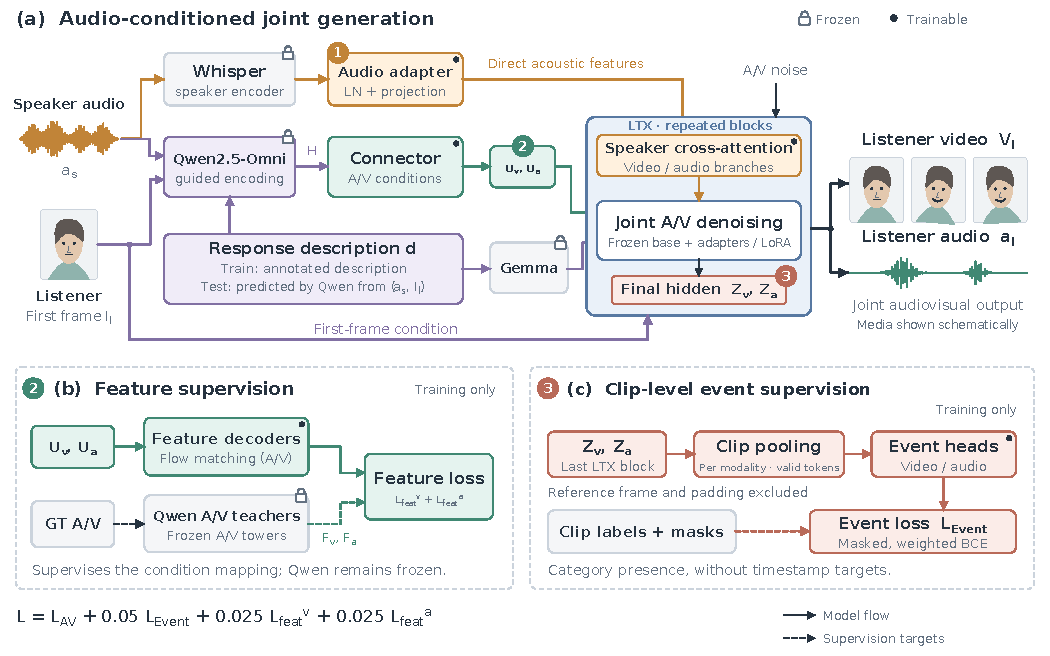
\includegraphics[width=\textwidth]{F3_method.pdf}
\caption{\figdraft{F3: Generation framework and training supervision} A connector maps guided Qwen representations to video and audio conditions, which are appended to Gemma text conditions. An independent Whisper path supplies speaker-audio features to both LTX streams. Feature supervision trains the condition mapping with frozen target-media features; clip-level Event supervision reads the final LTX block. Training uses annotated descriptions, whereas inference predicts and re-encodes descriptions from the permitted inputs. Both auxiliary objectives are used only during training. Portraits and waveforms are schematic.}
\label{fig:method}
\end{figure*}

\subsection{Overview}
\label{sec:conditioning}
\label{sec:task}
\paragraph{Task definition.}
Given the current speaker audio
$a_s$ and a listener reference
image $I_l$, we generate audiovisual
feedback as
\begin{equation}
    (\widehat V_l,\widehat a_l)
    = \mathcal{G}_{\Theta}(a_s,I_l),
    \label{eq:task}
\end{equation}
where $\mathcal{G}_{\Theta}$ denotes
the generation framework,
and $\widehat V_l$ and $\widehat
a_l$ are the listener video
and audio over the corresponding
interval.
We focus on feedback while the
speaker holds the conversational
floor, including facial expressions,
head movements, quiet
listening and brief
vocal acknowledgments.

\paragraph{Overview.}
Our framework uses a LoRA-adapted Qwen2.5-Omni
model~\cite{qwen25omni} to predict a reaction description $d$
from the speaker audio $a_s$ and listener image $I_l$.
The model then re-encodes these inputs together with $d$ to
obtain multilayer hidden states $H$, while
Gemma~\cite{gemma_pending} encodes the same description into
text conditions. A trainable connector $C_\theta$ maps $H$
into video and audio conditions:
\begin{equation}
    (U_v,U_a)=C_\theta(H),\qquad
    c_m=[G_m(d);U_m],\quad m\in\{v,a\},
    \label{eq:conditions}
\end{equation}
where $G_m(d)$ denotes the processed Gemma context for modality
$m$, and brackets denote token concatenation.

The concatenated conditions $c_v$ and $c_a$ enter the LTX
generator~\cite{ltx_pending} through its native text
cross-attention. A separate Whisper branch~\cite{whisper}
supplies direct speaker-audio features through additional
cross-attention in both generation streams. Together with
the listener reference image, these conditions guide the
joint generation of listener video and audio.

During generator training, the annotated reaction description
$d^*$ replaces the predicted description. Target audiovisual
feature supervision adapts the connector outputs $U_v$ and
$U_a$ to listener generation, while clip-level event supervision
acts on the final LTX hidden states to encourage the
corresponding feedback categories to occur.

At inference, Qwen predicts a reaction description $\hat d$
from $a_s$ and $I_l$, and then processes the original inputs
together with $\hat d$ to produce guided hidden states.
Gemma encodes the same description into text conditions.
Both conditions guide the subsequent audiovisual generation.

\subsection{Direct Speaker-Audio Conditioning}
\label{sec:direct-audio}
% Paragraph role P04: Whisper动机与设计——保留直接声学信息，补充描述与高层条件。
A reaction description summarizes intended behavior, but does not
explicitly preserve every local acoustic cue in the speaker's utterance.
We therefore provide a separate path from speaker audio to the generator.
A frozen Whisper-large-v3 encoder~\cite{whisper} extracts a
temporal feature sequence from the speaker audio. A trainable
LayerNorm and linear adapter map these features to speaker
context $S$. At each LTX block $b$, independent cross-attention
branches inject $S$ into the video and audio streams.
For modality $m\in\{v,a\}$, the attention computation within
each head is
\begin{equation}
\begin{aligned}
    Q_{b,m} &= \mathcal{P}^{Q}_{b,m}(h_{b,m}),\\
    K_{b,m} &= \mathcal{P}^{K}_{b,m}(S),\qquad
    V_{b,m} = \mathcal{P}^{V}_{b,m}(S),\\
    A_{b,m} &= \operatorname{softmax}\!\left(
        \frac{Q_{b,m}K_{b,m}^{\top}}{\sqrt{d_k}}
        +\mathcal{M}
    \right)V_{b,m},
\end{aligned}
\label{eq:speaker-attention}
\end{equation}
where $h_{b,m}$ denotes the generation hidden states,
$d_k$ is the head dimension, and $\mathcal{M}$ masks padded
speaker tokens.Queries and keys are normalized and augmented with temporal
RoPE before attention, while values are obtained by a linear
projection of the adapted speaker features $S$.

Temporal RoPE uses a common time origin in seconds for the
speaker and generation features. Leading and internal speaker
silence are retained. The multi-head attention outputs are
projected back into their respective streams and added
residually, with zero-initialized output projections.
The adapter and attention branches are optimized through
the audiovisual generation and event-supervision objectives.

\subsection{Target Audiovisual Feature Supervision}
\label{sec:feature}
% Paragraph role P06: Feature动机——让实际送入生成器的条件携带目标媒体信息。
The connector must transform general multimodal representations into
conditions useful for listener generation. To supervise this mapping,
we extract target features $F_v$ and $F_a$ from real listener video and
processed audio using frozen Qwen visual and audio encoders. 
For feature supervision, each condition token in $U_m$ is
paired with the corresponding target feature in $F_m$.
An auxiliary decoder $D_{\phi_m}$ for each modality learns
to recover target features conditioned on $U_m$, following the
AdaLN-modulated feature-decoder design of Bernini~\cite{bernini_pending}.

% Paragraph role P07: Feature公式——独立噪声下的特征流匹配，保留有效位置与安静音频。
For each valid feature position, we sample Gaussian noise $\epsilon$
and a noise level $\sigma\sim\mathcal U(0,1)$, forming
$x_{\sigma,m}=(1-\sigma)F_m+\sigma\epsilon$. The decoder predicts
the flow velocity toward noise, with objective
\begin{equation}
 \mathcal L_{\mathrm{Feature}}^m =
 \mathbb E_{\sigma,\epsilon}\!\left[
 \big\|D_{\phi_m}(x_{\sigma,m},\sigma,U_m)
       -(\epsilon-F_m)\big\|_{\Omega_m}^{2}\right].
\label{eq:feature}
\end{equation}
Here, $\Omega_m$ contains positions with valid target features
and conditioning tokens. For each sample, the error is averaged
over these positions and feature dimensions, and then averaged
across samples. Silent audio is retained as a valid target.

The auxiliary decoders and LTX share the same conditioning
representations $U_m$. Feature-loss gradients propagate through
the decoders to the connector, encouraging $U_m$ to capture
information relevant to the target listener audio and video.
The auxiliary decoders and target-feature encoders are used
only during training.

\subsection{Clip-Level Event Supervision}
\label{sec:event}
To explicitly supervise the presence of feedback categories,
we apply clip-level event supervision to the LTX generator.
The video and audio hidden states $Z_v$ and $Z_a$ from its
final Transformer block are pooled into a clip representation
for each modality. Video pooling averages spatial tokens
within each time step, followed by temporal averaging;
audio pooling averages over temporal positions.
Only valid generated positions participate in pooling,
excluding reference-frame and padding tokens.
Two modality-specific event heads then map the pooled
representations to clip-level category logits.

% Paragraph role P10: Event标签与公式——区分正例、弱负例和未知，按有效样本归一化。
Clip-level targets are extracted from reaction descriptions
using the checks described in \cref{sec:annotation}.
Each clip--category pair is assigned a positive label,
a weak negative, or an unknown status. Supported positives
receive weight 1. An unmentioned category receives
weak-negative weight 0.1 only when the description passes
the completeness checks. Uncertain or conflicting labels
are excluded from supervision.

For sample $i$ and category $c$, let $s_{ic}$ denote the
predicted logit, $y_{ic}$ the binary target, and $M_{ic}$
the validity mask. The sample weight $w_{ic}$ follows
the rules above. The event loss averages the weighted
classification error within each category and then
across valid categories:
\begin{equation}
    \mathcal L_{\mathrm{Event}}
    =
    \frac{1}{|\mathcal C_{\mathrm{eff}}|}
    \sum_{c\in\mathcal C_{\mathrm{eff}}}
    \frac{1}{N_c}
    \sum_i M_{ic}w_{ic}\,
    \mathrm{BCE}_{\alpha_c}(s_{ic},y_{ic}),
    \label{eq:event}
\end{equation}
where $N_c=\sum_i M_{ic}$ counts valid targets for category
$c$, and $\mathcal C_{\mathrm{eff}}$ contains enabled
categories with $N_c>0$. The positive-class weight
$\alpha_c$ is computed from training-label statistics
to account for class imbalance. Normalization by $N_c$
preserves the reduced contribution of weak negatives.

% Paragraph role P11: 整段监督动机——语境约束反馈方向，具体时序允许多种合理实现。
The current utterance provides cues about the affective or
attitudinal character of an appropriate response. 
%   For example, positive news may elicit smiling or shared laughter, while a
%   head shake can express disagreement. 
Even when conveying a
similar intent, listeners may react at different moments,
with different durations and repetition counts. A single
recorded response therefore represents only one plausible
temporal realization.

Motivated by this variability, our event objective supervises
the presence of feedback categories over the entire clip.
It explicitly encourages the annotated categories to occur
without prescribing their onset times, durations, or repetition
counts. This behavior-level supervision complements the
audiovisual objective, which continues to supervise the paired
listener audio and video.



\subsection{Training and Inference}
\label{sec:training}
\paragraph{Joint objective.}
% Paragraph role P12: AV目标——双路潜空间流匹配，固定参考首帧并屏蔽无效支持。
The audiovisual generator is trained with a flow-matching
objective. For each modality $m\in\{v,a\}$, a frozen VAE
encodes the target media into latents $x_0^m$. At generated
positions, Gaussian noise $\epsilon_m$ is added at a sampled
noise level $\tau$:
\begin{equation}
    x_\tau^m=(1-\tau)x_0^m+\tau\epsilon_m.
    \label{eq:av-noising}
\end{equation}

Conditioned on the inputs described above, LTX jointly
predicts video and audio velocities $\widehat v^m$,
with targets $\epsilon_m-x_0^m$. The audiovisual loss is
\begin{equation}
    \mathcal L_{\mathrm{AV}}
    =
    \mathbb E\!\left[
    \sum_{m\in\{v,a\}}
    \operatorname{MSE}_{\mathrm{valid}}
    \left(\widehat v^m,\epsilon_m-x_0^m\right)
    \right],
    \label{eq:av}
\end{equation}
where $\operatorname{MSE}_{\mathrm{valid}}$ averages the
squared error over valid generated latent positions and
feature dimensions. The reference-frame latent remains
fixed, and padding positions are excluded from the loss.



% Paragraph role P13: 总目标——Whisper是条件路径，Feature与Event是辅助监督。
The overall training objective combines audiovisual generation,
feature reconstruction, and event supervision:
\begin{equation}
\begin{aligned}
    \mathcal L ={}&
    \mathcal L_{\mathrm{AV}}
    +0.05\mathcal L_{\mathrm{Event}}\\
    &+0.025\sum_{m\in\{v,a\}}
    \mathcal L_{\mathrm{Feature}}^m.
\end{aligned}
\label{eq:total}
\end{equation}
This objective jointly optimizes the connector, Whisper
conditioning branch, LTX attention LoRA, and auxiliary
feature decoders and event heads.

\paragraph{Inference.}
Given $a_s$ and $I_l$, Qwen predicts a reaction description
$\hat d$ and processes it together with the original inputs
to obtain guided hidden states. The connector maps these
states to $U_v$ and $U_a$, while Gemma encodes $\hat d$
into text conditions and Whisper extracts speaker-audio
features. Using these conditions, LTX jointly samples video
and audio latents from noise while keeping the reference-frame
latent fixed. The sampled latents are then decoded into
listener video and audio. Sampling settings are provided
in \cref{sec:setup}.

\section{Listening Data Construction}
\label{sec:data}
% Section role: explain how paired media, descriptions, and labels are constructed.

\begin{figure*}[t]
\centering
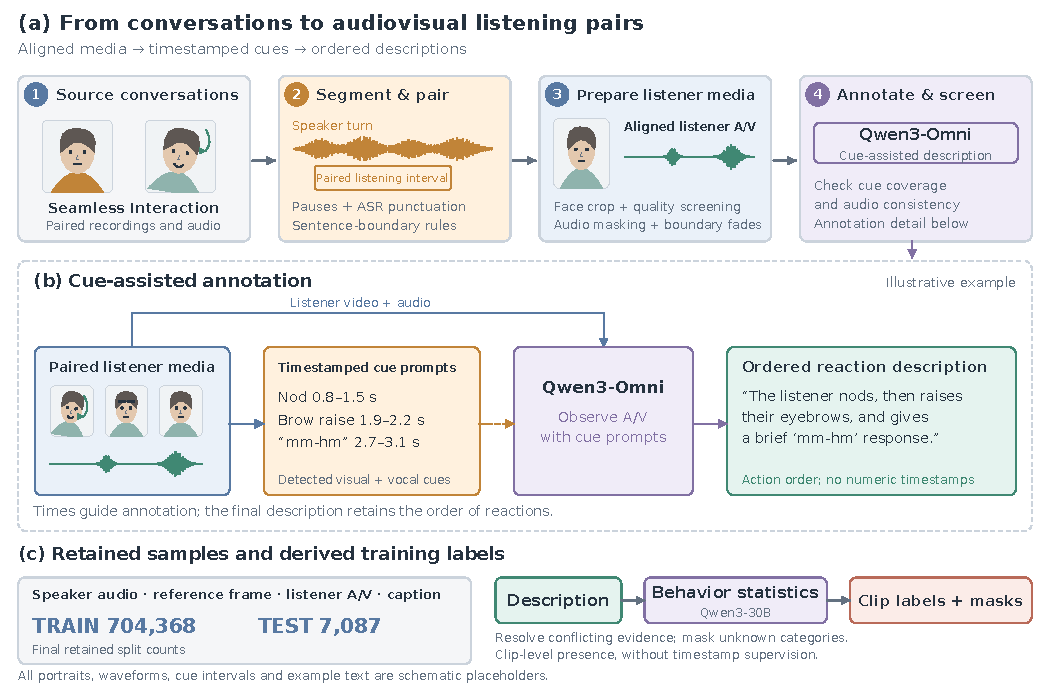
\includegraphics[width=\textwidth]{F2_data.pdf}
\caption{\figdraft{F2: Data construction and cue-assisted annotation} Seamless conversations are segmented and paired before listener media processing. Listener audiovisual media and timestamped reaction cues guide Qwen3-Omni to produce an ordered description without numerical timestamps. Each sample links the input conditions, listener targets, and description. Text-based behavior extraction and conflict masking produce clip-level training labels. Example media, cue intervals, and descriptions are schematic; the reported resource counts differ from the AV training selection.}
\label{fig:data}
\end{figure*}
\subsection{Role-Aware Pair Construction}
\label{sec:pairing}

We construct 2--12-second listening clips from Seamless
conversations~\cite{seamless}, pairing the current speaker's
audio with a listener reference frame and synchronized
listener audio and video. Transcripts, word timings,
speech activity, and pauses guide segmentation toward
complete sentences. Roles switch when the listener takes
the conversational floor, while brief vocal backchannels,
including overlapping feedback, remain part of listening.
\Cref{fig:data} summarizes the pipeline.

Listener videos are screened, corrected for orientation
where needed, and cropped consistently for reaction
detection and annotation. Listener audio is extracted
from the participant's separate track over the same
interval. Officially annotated vocal regions are retained
with short margins and boundary fades; the remaining
audio is set to zero, preserving duration and audiovisual
alignment.

\subsection{Cue-Assisted Reaction Annotation}
\label{sec:annotation}

To reduce omissions of brief reactions, we extract visual
and vocal cues and provide their categories and temporal
intervals to Qwen3-Omni~\cite{qwen3omni}, together with the
listener audio and video. The model is prompted to describe
the reactions in their observed order without numerical
timestamps.

We then use Qwen3-30B-A3B-Instruct-2507~\cite{qwen3} to
extract clip-level behavior labels from these descriptions.
Supported categories provide positive labels, while
unmentioned categories receive weak-negative labels only
after completeness checks. Uncertain or conflicting labels
are masked, as detailed in \cref{sec:event}.

\subsection{Dataset Statistics}
\label{sec:data-statistics}
% Paragraph role P07: 样本与规模
Each sample links the current speaker audio, the listener's first frame, aligned listener video and audio, and a reaction description, together with source and temporal metadata. The retained resource contains 704,368 training samples and 7,087 test samples. The AV generation model uses a separately selected training set, specified in \cref{sec:setup}; these counts do not denote the same training manifest. Data and annotation quality checks are organized in \cref{sec:validation}.
% Candidate 1: dataset comparison. Caption is below the table as requested.
% TBD means unverified in this writing pass, not unavailable or unreported.
\begin{table*}[t]
    \centering\small
    \begin{tabularx}{\textwidth}{@{}Yccc@{}}
    \toprule
    Dataset & \makecell{Listening\\organization} &
    \makecell{Separate speaker/\\listener audio} & Paired samples \\
    \midrule
    ViCo~\cite{vico} & Dedicated & \pending & 483 clips \\
    RealTalk~\cite{realtalk} & General dialogue & \pending & \pending \\
    Seamless~\cite{seamless} & General dialogue & \on & \pending \\
    SpeakerVid-5M (listening)~\cite{speakervid} & Dedicated branch & \off & \pending \\
    ResponseNet~\cite{omniresponse} & General dialogue & \on & 696 conversations \\
    GLARE~\cite{glare} & Dedicated & \pending & 107,149 clips \\
    \midrule
    Ours & Dedicated & \on & 711,455 clips \\
    \bottomrule
    \end{tabularx}
    \caption{【Candidate 1】Comparison of data resources. Separate audio denotes participant-specific tracks for both speakers and listeners; the SpeakerVid-5M listening branch pairs speaker audio with silent listener video. Conversation counts and segmented-clip counts use different units. Ours counts the retained training and test pairs.}
    \label{tab:dataset-comparison}
    \end{table*}
    

% Candidate 2: method scope and generated modalities, not a performance ranking.
\begin{table*}[t]
    \centering\small
    \begin{tabularx}{\textwidth}{@{}Yccc@{}}
    \toprule
    Method & \makecell{Listening\\modeling} & Joint A/V & Generated output \\
    \midrule
    CustomListener~\cite{customlistener} & Dedicated & \NA & Visual \\
    DiffListener~\cite{difflistener} & Dedicated & \NA & Visual \\
    GLARE~\cite{glare} & Dedicated & \NA & Visual \\
    INFP~\cite{infp} & Included & \NA & Visual \\
    OmniResponse~\cite{omniresponse} & Included & \off & Audio + visual \\
    OmniPersona~\cite{omnipersona} & Included & \on & Audio + visual \\
    \midrule
    Ours & Dedicated & \on & Audio + visual \\
    \bottomrule
    \end{tabularx}
    \caption{【Candidate 2】Comparison of generation settings. Dedicated methods focus on listening; Included methods also model listening within broader interaction tasks. Joint A/V denotes joint audio--video synthesis; OmniResponse synthesizes audio through TempoVoice. Outputs list generated modalities, excluding supplied audio.}
    \label{tab:method-comparison}
    \end{table*}
    

% Candidate 3: our retained train/test resource; not the 284,218-clip AV selection.
% Example category rows must be replaced/expanded after the vocabulary is frozen.
% Neither the training Event vocabulary nor the seven evaluation classes defines
% the full dataset taxonomy automatically. Counts below are intentionally TBD.
\begin{table*}[t]
    \centering\small
    \begin{tabularx}{\textwidth}{@{}lYrrr@{}}
    \toprule
    Modality & Behavior category & Train pairs & Test pairs & Total pairs \\
    \midrule
    Visual & Head nodding & \pending & \pending & \pending \\
           & Smiling & \pending & \pending & \pending \\
           & $\ldots$ & $\ldots$ & $\ldots$ & $\ldots$ \\
    Vocal & Audible laughter & \pending & \pending & \pending \\
          & $\ldots$ & $\ldots$ & $\ldots$ & $\ldots$ \\
    \midrule
    \multicolumn{2}{@{}l}{Number of visual categories} & \multicolumn{3}{r@{}}{\pending} \\
    \multicolumn{2}{@{}l}{Number of vocal categories} & \multicolumn{3}{r@{}}{\pending} \\
    \multicolumn{2}{@{}l}{Total number of categories} & \multicolumn{3}{r@{}}{\pending} \\
    \midrule
    \multicolumn{2}{@{}l}{All pairs (unique within each split)} & 704,368 & 7,087 & 711,455 \\
    \bottomrule
    \end{tabularx}
    \caption{【Candidate 3】Category distribution and split sizes of our retained data. Category rows illustrate the layout pending the final vocabulary and counts. Each pair is counted once per category and may contain multiple categories, so category counts need not sum to the dataset total.}
    \label{tab:data-statistics-candidate}
    \end{table*}
    
\cnnote{感觉可以去掉。如果保留的话要补充：数据总量xx条xxh、标柱类别数xx种}{}

\section{Experiments}
\label{sec:experiments}

\subsection{Experimental Setup}
\label{sec:setup}
\paragraph{Datasets.}
We train the audiovisual generator on 284,218 clips
(approximately 500 hours) selected from the Seamless
training and development splits. This selection differs
from the full resource reported in
\cref{sec:data-statistics}.
We evaluate audiovisual backchannel generation on
Seamless and ResponseNet, and visual listening reactions
on ViCo.

\paragraph{Implementation details.}
We use LTX-2.3-22B~\cite{ltx_pending} as the audiovisual
generator, Qwen2.5-Omni-3B~\cite{qwen25omni} as the reaction
planner, and Whisper-large-v3~\cite{whisper} for speaker
audio encoding. Videos are processed at $512\times512$
resolution and 25 FPS, and speaker audio is resampled to
16\,kHz for Whisper. The Qwen planner is separately
fine-tuned with LoRA rank 32 and scaling parameter 64.
For LTX, we apply LoRA with rank and scaling parameter 8
to its native attention and feed-forward layers, while
fully training the additional Whisper attention branches.

Generator training uses 31 NVIDIA H200 GPUs with one
clip per GPU, BF16 mixed precision, and gradient
checkpointing. We use AdamW with
$(\beta_1,\beta_2)=(0.9,0.999)$, $\epsilon=10^{-8}$,
and zero weight decay. Learning rates are $10^{-5}$
for LTX LoRA, $3\times10^{-5}$ for the connector,
Whisper conditioning branch, and feature decoders,
and $10^{-4}$ for the event heads. Training is configured
for 9,169 iterations with 50 warm-up steps.
The loss weights are specified in \cref{eq:total}.
At inference, we use 30 Euler sampling steps with
video and audio CFG scales of \pending.

% \cnnote{引用与配置待补}{上述结构及维度已按当前配置和实际复用源码核对。Gemma的正式模型版本、LTX与Bernini的正式书目信息仍需补齐；源码定位见配套方法核对文档。生成训练中的Qwen未做规划SFT。}
% \cnnote{采样设置待冻结}{中文稿当前共享推理函数采用30步采样，视频／音频CFG为3／7。它们是可在实验中统一调整的参数，不是方法贡献。最终检查点、规划器及采样协议须共同确定后填写。}
% \cnnote{版本待冻结}{当前生成训练使用base Qwen hidden；最新LTX6000／6500＋SFT2752评测由SFT模型预测描述并重新提取H，属于“训练base H、推理SFT H”的配置。若最终主表采用该版本，须说明规划SFT及条件切换，并在所有对照中统一；本轮不把SFT自动并入AV＋Whisper＋Feature＋Event的四项设计。最终检查点、规划器和预算仍需冻结，不同batch／步数的终点不能直接当作等预算。}

\paragraph{Baselines and benchmarks.}

\cnnote{待补充}{}
% \cnnote{完整AV候选}{优先安排本文A0／A1及Qwen2.5-Omni→OVI系统对照。后者需适配允许安静和短反馈，固定模型与prompt，不能使用真实caption、事件或listener音轨。OmniResponse、OmniPersona、SpeakerVid-5M目前尚未获得可执行原生成器，先保留文献比较，不复制原表分数到本文短pair表。}
% \cnnote{视觉与额外输入对照}{GLARE需重训并披露Tref及previous motion来源；DyStream将self audio置零，Avatar Forcing将self audio和user视觉置零。L2L、DualTalk等保留额外动作／音轨条件时单列表，纯动作结果只在同表示空间比较；未核验renderer前不纳入视频表。RLHG、DIM、ReactFace、ListenFormer、LFI为资源允许时的扩展，不全部列为必做。}
% \cnnote{共同协议}{统一片段范围、参考帧、分辨率／帧率、音量处理、采样预算和失败处理，不用GT挑best-of-N。OVI1.1单次上限10秒而本任务可达11.95秒，需选择全部方法的共同窗口或公开分段／拼接协议，不能只截短基线。}
% \cnnote{原论文数值}{原协议文献表与本地实测分开。BFM/L1、EMOCA／DECA距离和不同含义的FD不混排；各论文RealTalk划分不视为统一测试。官方权重迁移、本文重训、第三方重实现及引用分别标注；协议不一致不计算相对提升。FID/FVD使用统一特征汇总，不平均分片分数。}

% Metrics are defined once here; results below refer back to this protocol.
\subsection{Evaluation Protocol}
\label{sec:evaluation}

\paragraph{Clip-level event agreement.}
Valid listening reactions can occur at different times,
making strict alignment with a single reference overly
restrictive. We therefore compare event-category presence
over each clip, counting repeated occurrences only once.
We report macro-precision, macro-recall, and macro-F1
separately for visual and vocal categories with reference
positives, and report false-positive rates for the remaining
categories. These scores measure category agreement with
the observed response, complementing the assessment of
contextual appropriateness.

\paragraph{Audiovisual quality and behavior.}
Building on the OmniResponse evaluation
framework~\cite{omniresponse}, we measure video quality
using PSNR, SSIM, LPIPS, FID, and FVD.
Emo-Acc, Emo-Div, and $\Delta$Resp characterize expression
agreement, expression diversity, and listening-motion
differences, following AnyTalker~\cite{anytalker}.
Audio diagnostics measure activity-duration error,
missed vocal responses, excess vocal duration, and false
vocalization on silent clips. Where applicable, SyncNet's LSE-D and LSE-C
measure lip synchronization. Unsupported cases are
reported as N/A, together with valid evaluation coverage.

\paragraph{Human evaluation.}
Human evaluation targets contextual appropriateness,
naturalness and engagement, and audiovisual coordination
(\cref{sec:qualitative}). The assessment allows alternative
reasonable reactions and natural quiet listening.

\subsection{Quantitative Comparisons}
\label{sec:quantitative}
\paragraph{Audiovisual backchannel generation.}
% Paragraph role P05: 完整视听任务的比较范围
The full-task comparison concerns listener audio, visual reactions, and their coordination (\cref{tab:av}). It uses current speaker audio and a listener first frame as inputs and does not treat supplied listener audio as generated audio.
% \cnnote{比较所能支持的结论}{已知listener音轨的动画对照只评价驱动画面；独立OVI的共享预测文本对照评价生成器，Qwen→OVI端到端对照评价系统，两者均不替代三组件消融。不同训练来源的迁移结果不能解释为共同训练下的架构因果优势。}
% \cnnote{定量结果待写}{完成同协议比较后，先写主表支持的最重要发现，再说明对应的媒体质量、反馈类别和声音诊断证据；如指标有取舍，明确写出。当前不预设本文优于基线。}
\begin{table*}[t]
    \centering\small
    \setlength{\tabcolsep}{2pt}
    \renewcommand{\arraystretch}{1.1}
    \begin{tabularx}{\textwidth}{@{}Y*{16}{r}@{}}
    \toprule
    & \multicolumn{6}{c}{Visual quality}
    & \multicolumn{4}{c}{Feedback behavior}
    & \multicolumn{3}{c}{Visual events}
    & \multicolumn{3}{c}{Audio events} \\
    \cmidrule(lr){2-7}
    \cmidrule(lr){8-11}
    \cmidrule(lr){12-14}
    \cmidrule(lr){15-17}
    Method
    & \makecell{CPBD\\$\uparrow$}
    & \makecell{PSNR\\$\uparrow$}
    & \makecell{SSIM\\$\uparrow$}
    & \makecell{FID\\$\downarrow$}
    & \makecell{FVD\\$\downarrow$}
    & \makecell{LPIPS\\$\downarrow$}
    & \makecell{Emo-Acc\\$\uparrow$}
    & Emo-Div
    & \makecell{$\Delta$Resp\\$\downarrow$}
    & \makecell{MLLM\\RDR}
    & \makecell{P\\$\uparrow$}
    & \makecell{R\\$\uparrow$}
    & \makecell{mF1\\$\uparrow$}
    & \makecell{P\\$\uparrow$}
    & \makecell{R\\$\uparrow$}
    & \makecell{mF1\\$\uparrow$} \\
    \midrule
    L2L~\cite{learningtolisten}
    & \pending & \pending & \pending & \pending & \pending &
    \pending
    & \pending & \pending & \pending & \pending
    & \pending & \pending & \pending
    & \NA & \NA & \NA \\
  
    DIM~\cite{dim}
    & \pending & \pending & \pending & \pending & \pending &
    \pending
    & \pending & \pending & \pending & \pending
    & \pending & \pending & \pending
    & \NA & \NA & \NA \\
  
    ViCo~\cite{vico}
    & \pending & \pending & \pending & \pending & \pending &
    \pending
    & \pending & \pending & \pending & \pending
    & \pending & \pending & \pending
    & \NA & \NA & \NA \\
  
    ListenFormer~\cite{listenformer}
    & \pending & \pending & \pending & \pending & \pending &
    \pending
    & \pending & \pending & \pending & \pending
    & \pending & \pending & \pending
    & \NA & \NA & \NA \\
  
    DyStream~\cite{dystream}
    & \pending & \pending & \pending & \pending & \pending &
    \pending
    & \pending & \pending & \pending & \pending
    & \pending & \pending & \pending
    & \NA & \NA & \NA \\
  
    GLARE~\cite{glare}
    & \pending & \pending & \pending & \pending & \pending &
    \pending
    & \pending & \pending & \pending & \pending
    & \pending & \pending & \pending
    & \NA & \NA & \NA \\
  
    Avatar Forcing~\cite{avatarforcing}
    & \pending & \pending & \pending & \pending & \pending &
    \pending
    & \pending & \pending & \pending & \pending
    & \pending & \pending & \pending
    & \NA & \NA & \NA \\

    Qwen2.5-Omni + LTX~\cite{avatarforcing}
    & \pending & \pending & \pending & \pending & \pending &
    \pending
    & \pending & \pending & \pending & \pending
    & \pending & \pending & \pending
    & \NA & \NA & \NA \\
    \midrule
    Ours
    & \pending & \pending & \pending & \pending & \pending &
    \pending
    & \pending & \pending & \pending & \pending
    & \pending & \pending & \pending
    & \pending & \pending & \pending \\
    \bottomrule
    \end{tabularx}
    \caption{Generation quality and feedback behavior comparison
    on [seamless dataset]. MLLM-RDR denotes the MLLM-based reaction
    detection rate. Event P, R, and mF1 are macro-averaged
    using clip-level category presence. Audio-event metrics
    are N/A for methods without generated audio.}
    \label{tab:av}
    \end{table*}

\paragraph{Shared visual-listening capabilities.}
% Paragraph role P06: 视觉对照与额外输入边界
The visual comparison concerns capabilities shared with video-only listening methods (\cref{tab:visual}). Methods that require additional inputs or produce only motion are considered separately; their results do not establish performance on the full audiovisual task.
\begin{table*}[t]
    \centering\small
    \setlength{\tabcolsep}{3pt}
    \begin{tabularx}{\textwidth}{@{}Yrrrrrrrrrr@{}}
    \toprule
    & \multicolumn{4}{c}{Feedback behavior}
    & \multicolumn{3}{c}{Visual events}
    & \multicolumn{3}{c}{Audio events} \\
    \cmidrule(lr){2-5}
    \cmidrule(lr){6-8}
    \cmidrule(lr){9-11}
    Method
    & \makecell{Emo-Acc\\$\uparrow$}
    & Emo-Div
    & \makecell{$\Delta$Resp\\$\downarrow$}
    & \makecell{MLLM\\RDR}
    & P$\uparrow$
    & R$\uparrow$
    & mF1$\uparrow$
    & P$\uparrow$
    & R$\uparrow$
    & mF1$\uparrow$ \\
    \midrule
    L2L~\cite{learningtolisten}
    & \pending & \pending & \pending & \pending
    & \pending & \pending & \pending
    & \NA & \NA & \NA \\
    DIM~\cite{dim}
    & \pending & \pending & \pending & \pending
    & \pending & \pending & \pending
    & \NA & \NA & \NA \\
    ViCo (RLHG)~\cite{vico}
    & \pending & \pending & \pending & \pending
    & \pending & \pending & \pending
    & \NA & \NA & \NA \\
    ListenFormer~\cite{listenformer}
    & \pending & \pending & \pending & \pending
    & \pending & \pending & \pending
    & \NA & \NA & \NA \\
    DyStream~\cite{dystream}
    & \pending & \pending & \pending & \pending
    & \pending & \pending & \pending
    & \NA & \NA & \NA \\
    GLARE~\cite{glare}
    & \pending & \pending & \pending & \pending
    & \pending & \pending & \pending
    & \NA & \NA & \NA \\
    Avatar Forcing~\cite{avatarforcing}
    & \pending & \pending & \pending & \pending
    & \pending & \pending & \pending
    & \NA & \NA & \NA \\
    \midrule
    Ours
    & \pending & \pending & \pending & \pending
    & \pending & \pending & \pending
    & \pending & \pending & \pending \\
    \bottomrule
    \end{tabularx}
    \caption{待确定 Feedback behavior comparison on [vico dataset].
    MLLM-RDR denotes the MLLM-based reaction detection rate.
    Event precision, recall, and F1 are macro-averaged separately
    for visual and audio categories using clip-level presence,
    without requiring temporal overlap with reference events.
    Emo-Div measures expression diversity without a preferred
    direction.}
    \label{tab:visual}
    \end{table*}

\subsection{Qualitative Results and Human Evaluation}
\label{sec:qualitative}
\paragraph{Qualitative comparisons.}
% \cnnote{样例计划}{图F5先放可替换布局。后续按预先说明的规则选择合理安静倾听、动作与短声共同表达、遗漏或不适当失败三类。每例保留speaker原音频、listener首帧、一个真实参考、各方法帧序列及各自音轨；同一时刻展示不代表必须与GT同时反应。动作标签说明人工／自动来源。完整视频待插入，不能只看波形判断类别与音质。}
\begin{figure*}[t]
\centering
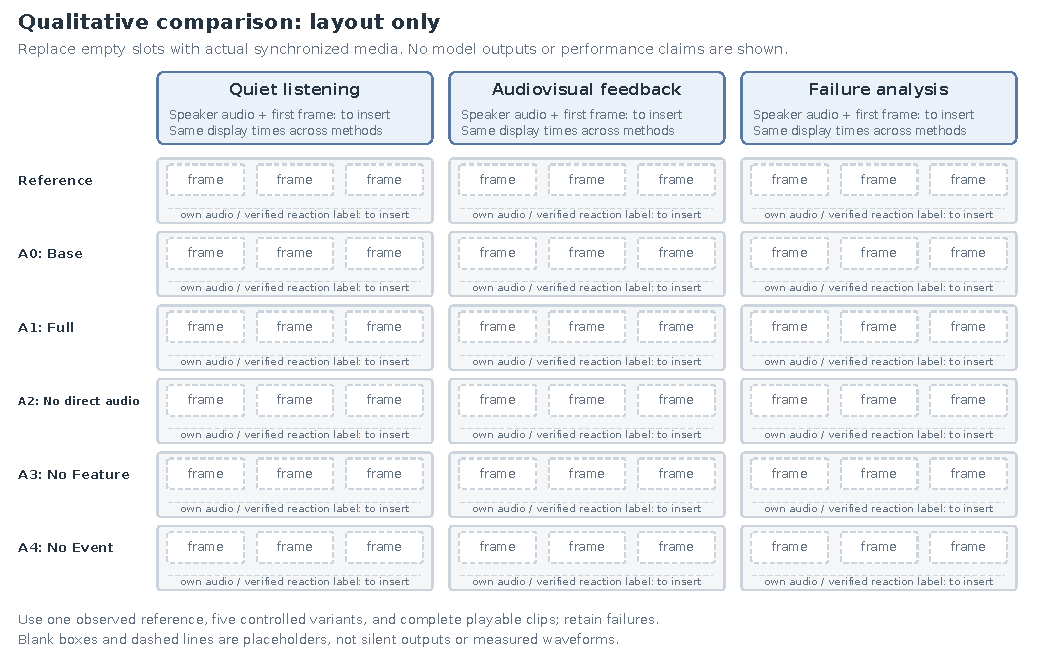
\includegraphics[width=\textwidth]{F5_results_layout.pdf}
\caption{\figdraft{F5: Qualitative comparison layout only} Three planned cases cover quiet listening, audiovisual feedback, and failure analysis. Rows reserve space for a reference response and the five ablation configurations. Every frame and audio slot is empty: this figure contains no generated result or claimed performance difference.}
\label{fig:qualitative}
\end{figure*}

\paragraph{Human evaluation.}
% \cnnote{人工评价计划}{在相同当前speaker音频与listener首帧条件下，匿名随机排序并由多位评分者判断适当性、参与感／自然度与声画协调（\cref{tab:human}）。画面／声音技术质量可分开评分。参考回应不是唯一正确答案，合理安静允许存在；无发声样本的相关协调项按协议记N/A并报告覆盖。人工仍需检查反应抢先、拖长或内部矛盾，不要求复现唯一GT时刻。}
% \cnnote{统计计划}{使用配对设计，按来源对话处理片段相关性，报告置信区间与有效样本。单次生成seed如实注明；样本bootstrap不替代训练多seed的不确定性。评分人数、量表／A-B形式及一致性统计待确定，不能预设自动指标与人评高度相关。}
 \begin{table*}[t]
    \centering\small
    \begin{tabularx}{\textwidth}{@{}Yccc@{}}
    \toprule
    Method
    & \makecell{Contextual\\appropriateness}
    & \makecell{Engagement /\\naturalness}
    & \makecell{Audiovisual\\coordination} \\
    \midrule
    Qwen+LTX
    & \pending & \pending & \pending \\
    GLARE
    & \pending & \pending & \NA \\
    DyStream
    & \pending & \pending & \NA \\
    Avatar Forcing
    & \pending & \pending & \NA \\
    Ours
    & \pending & \pending & \NA \\
    \bottomrule
    \end{tabularx}
    \caption{Human evaluation of contextual appropriateness,
    engagement and naturalness, and audiovisual coordination.
    Audiovisual coordination is not applicable to visual-only
    methods.}
    \label{tab:human}
    \end{table*}

\subsection{Ablation Studies}
\label{sec:ablation}

The full model combines the AV objective with Whisper
conditioning (W), clip-level event supervision (E),
and audiovisual feature supervision (F).
\Cref{tab:ablation} compares this model with three
variants: w/o W, w/o E, and w/o F. All configurations
retain the AV objective and Qwen/Gemma conditions.

These comparisons examine the contribution of direct
speaker-audio conditioning, event supervision for
feedback-category expression, and feature supervision
for adapting the conditioning representations to
listener audiovisual generation.

 \begin{table*}[t]
    \centering\small
    \begin{tabularx}{\textwidth}{@{}Ycccrrrrrr@{}}
    \toprule
    Configuration
    & W & F & E
    & FID$\downarrow$
    & FVD$\downarrow$
    & \makecell{Visual\\mF1$\uparrow$}
    & \makecell{Audio\\mF1$\uparrow$}
    & \makecell{Miss$\downarrow$\\(\%)}
    & \makecell{False$\downarrow$\\(\%)} \\
    \midrule
    Ours
    & \on & \on & \on
    & \pending & \pending & \pending
    & \pending & \pending & \pending \\
    \midrule
    w/o Whisper
    & \off & \on & \on
    & \pending & \pending & \pending
    & \pending & \pending & \pending \\
  
    w/o Feature
    & \on & \off & \on
    & \pending & \pending & \pending
    & \pending & \pending & \pending \\
  
    w/o Event
    & \on & \on & \off
    & \pending & \pending & \pending
    & \pending & \pending & \pending \\
    \bottomrule
    \end{tabularx}
    \caption{Component ablations.
    W denotes Whisper conditioning, F denotes audiovisual
    feature supervision, and E denotes clip-level event
    supervision on LTX hidden states. All configurations
    retain Qwen/Gemma conditioning and the AV objective.}
    \label{tab:ablation}
    \end{table*}
% \cnnote{受控条件与证据}{固定数据、标签、初始化、规划器、训练样本展示量和采样；可预生成同一预测描述供五组共用。训练仍用标注描述，测试用预测描述；GT描述对照另标oracle。W不能只用画质证明语义／韵律利用，F不能只用teacher重建损失证明最终媒体改善，E须同时看P/R/F1、误触发和合理安静倾听。}
% \cnnote{历史结果与扩展}{旧U-Event的6000／8000和新LTX6000＋SFT2752结果均不能代替这五组正式同条件结果。监督位置、整段／时序、两路Feature拆分和权重网格暂列可选；只有新增相应独立主张时再安排对照。}


\subsection{Data and Evaluation Validation}
\label{sec:validation}
\paragraph{Data and annotation quality.}
Validation protocols and quantitative checks remain \pending.
% \cnnote{资源与媒体抽检计划}{统计来源、角色、音轨、片段长度、人脸质量、有声／安静比例、逐类支持与共现。代表性随机抽检覆盖边界完整性、角色对应、音轨污染／过度截除和脸部可用性；稀有层过采样需按真实分布加权。资源分支关系放附录，正文保持最终规模简洁。}
% \cnnote{配对标注核验计划}{固定同批片段、Qwen3-Omni版本、采样设置与输出要求，比较仅音视频与加入带时间线索的匿名描述（\cref{tab:annotation}）。独立人工核验遗漏、无依据添加、顺序与发声内容；同时报告正确性和完整性。已有24条有声试点只能说明观察来源。若要声称数据处理提升生成效果，另需固定模型、规模和预算的训练对照。}
% \begin{table*}[t]
\centering\small
\caption{辅助标注质量表草案（待实施，可移至附录）。固定相同片段，对匿名描述进行独立人工核验；所有数值待填。}
\label{tab:annotation}
\begin{tabularx}{\textwidth}{@{}Yrrrrr@{}}
\toprule
标注设置 & 样本数 & 事件遗漏$\downarrow$ & 无依据添加$\downarrow$ & 顺序错误$\downarrow$ & 发声描述错误$\downarrow$ \\
\midrule
仅音视频 & \pending & \pending & \pending & \pending & \pending \\
音视频＋带时间反应线索 & \pending & \pending & \pending & \pending & \pending \\
\bottomrule
\end{tabularx}
\cnnote{统计口径待补}{各项分母、判定标准和分层抽样方式需先定义。检测线索不是人工真值；更长描述不直接表示更准确。媒体质量抽检另记录角色／切分合格率、音轨问题和脸部可用性。}
\end{table*}


% \paragraph{Event-evaluator reliability.}
% \cnnote{事件评测器核验}{在真实和生成媒体上分别抽样核验外部检测器，覆盖有声／无声、常见／稀有类及失败例；报告逐类质量、支持数和覆盖。训练弱负例不直接当测试负真值，未知／失败不当正确安静；不能用训练Event头自评。}
% \cnnote{本小节作用}{这里核验数据与测量工具是否可信；生成效果由主对比和消融回答，用户感受由前述人工评价回答。完成核验后报告具体发现，详细错误清单和逐类结果可放补充材料。}
% \cnnote{可选扩展与范围}{Whisper置零／错配、GT描述oracle、多seed、时长／发声／脸部质量分层和完整推理开销仅为可选诊断。错配可能产生条件冲突，不能单独证明理解；多样性需同时看适当性，不选best-of-N。推理开销包括描述、重编码、各编码器、生成与解码，不将片段吞吐叫流式延迟。本阶段不增加多轮历史、persona保持、全身或实时流式主张。}
% \cnnote{已有证据状态，按中文稿快照}{ViCo43已完成历史联合8000、DyStream和Avatar Forcing自动比较，人工评分为0；双200 LTX6000＋SFT2752有视频与活动结果，UTMOSv2无有效窗口，SyncNet／GLARE未运行；基础AV训练已启动，不能称五组完成。上述记录仅作筹备依据，当前不填正式结果表。}

\section{Conclusion}
\label{sec:conclusion}
% \cnnote{结论待写}{正式结果尚未汇齐。完成主对比、五组消融、数据质量及评价核验后，再根据实际证据写结论；当前不新增性能、泛化或交互体验提升的结论。}
\paragraph{Limitations and future work.}
% \cnnote{局限段落待写}{结果确定后，用一个短段落结合失败例说明适用边界。当前设定只使用当前语音与首帧；自动标注、外部事件检测及单一参考评价的局限需结合核验结果说明。这里不新增多轮历史、人物长期一致性或实时流式实验要求。}
% \cnnote{作者自查}{贡献：保留数据、模型和评价三条方向，效果证据待补。写作：已区分标注／生成模型、训练／推理描述和两类事件协议。实验：五组已规划，成绩留空。评价：外部检测、人工规范和覆盖待落实。方法：冻结基座及梯度路径已说明，版本与细节待核对。完整逐项核对见review/含义与证据核对.md。}

\clearpage
{\small\bibliographystyle{ieeenat_fullname}\bibliography{references}}
\end{document}
